\newpage
\section{SCD}
\thispagestyle{fancy}


\gls{SCD} utgjer grunnlaget for det meste av programmeringsdokumentasjonen i oppgåva vår.
Diagrammet er delt opp sidevegs og sekvensvis og viser styring mellom program og komponentar i kvar enkelt sekvens,
samt ei side for resterande felles styring.

Prosessen i \gls{SCD}en (blå linjer) er basert på \gls{PID} som blei laga etter gjennomgangen av anlegget i kapittel \ref{sec:6}.
\gls{SCD} tar omsyn til programmerbart utstyr og har derfor ikkje med manuelle ventilar, tilbakeslagsventilar eller liknande.

For å representere våre eigne funksjonsblokker var vi nøydde til å legge dei til i \gls{SCD}en.
\gls{SCD} verktøyet hadde moglegheit for å legge inn eigendefinerte blokker med respektive inngangar og utgangar.

Våre funksjonsblokker og \gls{IEC} funksjonstemplata i diagrammet er dei same blokkene som vi har laga og brukt i programmeringsdelen. 
Dei stipla linjene viser koplingar og styringa mellom dei. \newline
I enkelte av diagramma førte antall stipla linjer til at diagrammet vart vanskeleg å lese. Vi nytta oss derfor av koplingar med
unik ID for å illustrere tilknytinga.

Våre tilstanslogikkblokker har fått eigne forkortingar i \gls{SCD}en,  og dette er dei relevante forkortingane 
for å forstå blokkene og diagrammet.

\begin{itemize}
    \item \textbf{SM}:   State machine
    \item \textbf{FBP}:  Function Block Pause
    \item \textbf{FBI}:  Function Block Innpumping
    \item \textbf{FBR}:  Fucntion Block Reaksjon
    \item \textbf{FBS}:  Function Block Sedimentering
    \item \textbf{FBU}:  Function Block Uttapping
    \item \textbf{FBPH}: Function Block Pumpehus
\end{itemize}

Heile \gls{SCD} er tilgjengelig i vedlegg. (Vedlegg H). \newline
\newpage

\begin{tikzpicture}[remember picture, overlay]
    % Include the PDF page rotated, positioned at the center of the page
    \node[inner sep=0pt] at (current page.center) {
        \includegraphics[page=2,angle=90, scale=0.36, keepaspectratio]{Bilder/SCD.pdf}
    };

    % Place the caption at the bottom of the page
    \node[anchor=south, yshift=10mm] at (current page.south) { % Adjust yshift to position the caption
        \begin{minipage}{\textwidth}
            \centering
            \captionof{figure}{SCD av innpumpingssekvens}
            \label{fig:SCD}
        \end{minipage}
    };
\end{tikzpicture}
